% Options for packages loaded elsewhere
\PassOptionsToPackage{unicode}{hyperref}
\PassOptionsToPackage{hyphens}{url}
%
\documentclass[
  ignorenonframetext,
]{beamer}
\usepackage{pgfpages}
\setbeamertemplate{caption}[numbered]
\setbeamertemplate{caption label separator}{: }
\setbeamercolor{caption name}{fg=normal text.fg}
\beamertemplatenavigationsymbolsempty
% Prevent slide breaks in the middle of a paragraph
\widowpenalties 1 10000
\raggedbottom
\setbeamertemplate{part page}{
  \centering
  \begin{beamercolorbox}[sep=16pt,center]{part title}
    \usebeamerfont{part title}\insertpart\par
  \end{beamercolorbox}
}
\setbeamertemplate{section page}{
  \centering
  \begin{beamercolorbox}[sep=12pt,center]{part title}
    \usebeamerfont{section title}\insertsection\par
  \end{beamercolorbox}
}
\setbeamertemplate{subsection page}{
  \centering
  \begin{beamercolorbox}[sep=8pt,center]{part title}
    \usebeamerfont{subsection title}\insertsubsection\par
  \end{beamercolorbox}
}
\AtBeginPart{
  \frame{\partpage}
}
\AtBeginSection{
  \ifbibliography
  \else
    \frame{\sectionpage}
  \fi
}
\AtBeginSubsection{
  \frame{\subsectionpage}
}
\usepackage{amsmath,amssymb}
\usepackage{iftex}
\ifPDFTeX
  \usepackage[T1]{fontenc}
  \usepackage[utf8]{inputenc}
  \usepackage{textcomp} % provide euro and other symbols
\else % if luatex or xetex
  \usepackage{unicode-math} % this also loads fontspec
  \defaultfontfeatures{Scale=MatchLowercase}
  \defaultfontfeatures[\rmfamily]{Ligatures=TeX,Scale=1}
\fi
\usepackage{lmodern}
\ifPDFTeX\else
  % xetex/luatex font selection
\fi
% Use upquote if available, for straight quotes in verbatim environments
\IfFileExists{upquote.sty}{\usepackage{upquote}}{}
\IfFileExists{microtype.sty}{% use microtype if available
  \usepackage[]{microtype}
  \UseMicrotypeSet[protrusion]{basicmath} % disable protrusion for tt fonts
}{}
\makeatletter
\@ifundefined{KOMAClassName}{% if non-KOMA class
  \IfFileExists{parskip.sty}{%
    \usepackage{parskip}
  }{% else
    \setlength{\parindent}{0pt}
    \setlength{\parskip}{6pt plus 2pt minus 1pt}}
}{% if KOMA class
  \KOMAoptions{parskip=half}}
\makeatother
\usepackage{xcolor}
\newif\ifbibliography
\usepackage{graphicx}
\makeatletter
\def\maxwidth{\ifdim\Gin@nat@width>\linewidth\linewidth\else\Gin@nat@width\fi}
\def\maxheight{\ifdim\Gin@nat@height>\textheight\textheight\else\Gin@nat@height\fi}
\makeatother
% Scale images if necessary, so that they will not overflow the page
% margins by default, and it is still possible to overwrite the defaults
% using explicit options in \includegraphics[width, height, ...]{}
\setkeys{Gin}{width=\maxwidth,height=\maxheight,keepaspectratio}
% Set default figure placement to htbp
\makeatletter
\def\fps@figure{htbp}
\makeatother
\setlength{\emergencystretch}{3em} % prevent overfull lines
\providecommand{\tightlist}{%
  \setlength{\itemsep}{0pt}\setlength{\parskip}{0pt}}
\setcounter{secnumdepth}{-\maxdimen} % remove section numbering
%\usetheme{metropolis}


%\setbeamercolor{normal text}{bg=white}
%\addtobeamertemplate{frametitle}{}{\vspace{-0.5em}} % decrease
%\setbeamersize{text margin left=5mm,text margin right=10mm}
%\usefonttheme[onlymath]{serif}
%\usefonttheme{professionalfonts}
%%%%%%%%%%%%%%%%
% Packages
%%%%%%%%%%%%%%%%

\usepackage{geometry}
\usepackage{graphicx}
\usepackage{amssymb}
\usepackage{amsopn}
\usepackage{cancel}
\usepackage{epstopdf}
\usepackage{amsmath}  	% this permits text in eqnarray among other benefits
\usepackage{url}		% produces hyperlinks
\usepackage{hyperref}	% allows for color usage in tables
\usepackage[english]{babel}
%\usepackage[latin1]{inputenc}
\usepackage{colortbl}	% allows for color usage in tables
\usepackage{multirow}	% allows for rows that span multiple rows in tables
\usepackage{color}		% this package has a variety of color options
\usepackage{xcolor}
\usepackage{pgf}
\usepackage{calc}
\usepackage{ulem}
\usepackage{multicol}
\usepackage{booktabs}
\usepackage{textcomp}
%\usepackage[misc]{ifsym} % for the dice symbol \Cube{}
%\usepackage{txfonts}
%\usepackage{listings}
%\usepackage{tikz}
\usepackage{array}
\usepackage{wasysym}
\usepackage{fancyvrb}

%% change fontsize of R code
\ifdefined\Shaded
\let\oldShaded\Shaded
\let\endoldShaded\endShaded
\renewenvironment{Shaded}{\footnotesize\oldShaded}{\endoldShaded}
\fi
%% change fontsize of output
\let\oldverbatim\verbatim
\let\endoldverbatim\endverbatim
\renewenvironment{verbatim}{\footnotesize\oldverbatim}{\endoldverbatim}

%%%%%%%%%%%%%%%%
% Remove navigation symbols
%%%%%%%%%%%%%%%%

\setbeamertemplate{navigation symbols}{}

\setbeamertemplate{footline}[frame number]

%%%%%%%%%%%%%%%%
% User defined colors
%%%%%%%%%%%%%%%%

\xdefinecolor{oiB}{rgb}{0.22,0.52,0.72}
\definecolor{oiG}{rgb}{.298,.447,.114}
\xdefinecolor{hlblue}{rgb}{0.051,0.65,1}
\xdefinecolor{gray}{rgb}{0.5, 0.5, 0.5}
\xdefinecolor{darkGray}{rgb}{0.3, 0.3, 0.3}
\xdefinecolor{darkerGray}{rgb}{0.2, 0.2, 0.2}
\xdefinecolor{rubineRed}{rgb}{0.89,0,0.30}
\xdefinecolor{irishGreen}{rgb}{0,0.60,0}	
\definecolor{lightGreen}{rgb}{0.387,0.581,0.148}

%%%%%%%%%%%%%%%%
% Template colors
%%%%%%%%%%%%%%%%

%\setbeamercolor*{palette primary}{fg=white,bg= oiB!80!black!90}
%\setbeamercolor*{palette secondary}{fg=black,bg= oiB!80!black}
%\setbeamercolor*{palette tertiary}{fg=white,bg= oiB!80!black!80}
%\setbeamercolor*{palette quaternary}{fg=white,bg= oiB}
%\setbeamercolor{structure}{fg= oiB}
%\setbeamercolor{frametitle}{bg= oiB!90}
%\setbeamertemplate{blocks}[shadow=false]
%\setbeamersize{text margin left=2em,text margin right=2em}

%\setbeamercolor{code body}{bg=gray!20!white!80,fg=black}


%%%%%%%%%%%%%%%%
% Get rid of fancy enumerated list bullets
%%%%%%%%%%%%%%%%

%\setbeamertemplate{enumerate items}[default]

%%%%%%%%%%%%%%%%
% Custom commands
%%%%%%%%%%%%%%%%

\newcommand{\Sum}{\sum\nolimits}
\newcommand{\Hide}[2]{\underline{~~~\onslide<#1>{\alert{#2}}~~~}}
\newcommand{\hide}[2]{\underline{~~\onslide<#1>{\alert{#2}}~~}}
\newcommand{\hid}[2]{\onslide<#1>{\alert{#2}}}
\newcommand{\code}[1]{\textcolor{blue}{\texttt{#1}}}

% red
\newcommand{\red}[1]{\textit{\textcolor{rubineRed}{#1}}}

% pink
\newcommand{\pink}[1]{\textit{\textcolor{rubineRed!90!white!50}{#1}}}

% green
\newcommand{\green}[1]{\textit{\textcolor{irishGreen}{#1}}}

% orange
\newcommand{\orange}[1]{\textit{\textcolor{orange}{#1}}}

% links: webURL, webLin, appLink
\newcommand{\webURL}[1]{\urlstyle{same}{ \textit{\textcolor{darkGray}{\url{#1}}}}}
\newcommand{\webLink}[2]{\href{#1}{\textcolor{darkGray}{{#2}}}}
\newcommand{\appLink}[2]{\href{#1}{\textcolor{white}{{#2}}}}

% mail
\newcommand{\mail}[1]{\href{mailto:#1}{\textit{\textcolor{darkGray}{#1}}}}

% highlighting: hl, hlGr, mathhl
\newcommand{\hl}[1]{\textit{\textcolor{hlblue}{#1}}}
\newcommand{\hlGr}[1]{\textit{\textcolor{lightGreen}{#1}}}
\newcommand{\mathhl}[1]{\textcolor{hlblue}{\ensuremath{#1}}}

% two col: two columns
\newenvironment{twocol}[4]{
\begin{columns}[c]
\column{#1\textwidth}
#3
\column{#2\textwidth}
#4
\end{columns}
}





%%%%%%%%%%%%%%%%
% Change margin
%%%%%%%%%%%%%%%%

\newenvironment{changemargin}[2]{%
\begin{list}{}{%
\setlength{\topsep}{0pt}%
\setlength{\leftmargin}{#1}%
\setlength{\rightmargin}{#2}%
\setlength{\listparindent}{\parindent}%
\setlength{\itemindent}{\parindent}%
\setlength{\parsep}{\parskip}%
}%
\item}{\end{list}}

%%%%%%%%%%%%%%%%
% Footnote
%%%%%%%%%%%%%%%%

\long\def\symbolfootnote[#1]#2{\begingroup%
\def\thefootnote{\fnsymbol{footnote}}\footnote[#1]{#2}\endgroup}

%%%%%%%%%%%%%%%%
% Graphics
%%%%%%%%%%%%%%%%

\DeclareGraphicsRule{.tif}{png}{.png}{`convert #1 `dirname #1`/`basename #1 .tif`.png}



\setbeamercolor{normal text}{bg=white}

\DeclareMathOperator{\var}{var}
\newcommand{\boxmodel}[1]{\begin{array}{|c|}#1\\[2pt]\hline\end{array}}
\newcommand{\BXX}[2]{\begin{array}{|@{\,}c@{\,}|@{\,}c@{\,}|}\hline#1&#2\\[-1pt]\hline\end{array}}
\newcommand{\p}{\mathrm{P}}
\newcommand{\SE}{\mathrm{SE}}
\newcommand{\xbar}{\overline{x}}
\newcommand{\Xbar}{\overline{X}}
\newcommand{\ybar}{\overline{y}}
\newcommand{\Ybar}{\overline{Y}}
\newcommand{\zbar}{\overline{z}}
\newcommand{\Zbar}{\overline{Z}}
\newcommand{\wbar}{\overline{w}}
\newcommand{\Wbar}{\overline{W}}
\newcommand{\vbar}{\overline{v}}
\newcommand{\Vbar}{\overline{V}}
\newcommand{\dbar}{\overline{d}}
\newcommand{\Dbar}{\overline{D}}
\newcommand{\ebar}{\overline{e}}
\newcommand{\ehat}{\widehat{\epsilon}}
\newcommand{\yhat}{\widehat{y}}
\newcommand{\Yhat}{\widehat{Y}}
\newcommand{\bhat}{\widehat{\beta}}
\newcommand{\dl}[1]{\widehat{\delta}_{#1}}
\newcommand{\g}[1]{\widehat{\gamma}_{#1}}
\newcommand{\al}[1]{\widehat{\alpha}_{#1}}
\newcommand{\Bj}{{\beta_j}}
\newcommand{\Bp}{{\beta_p}}
\newcommand{\Bq}{{\beta_q}}
\renewcommand{\b}[1]{\widehat{\beta}_{#1}}
\newcommand{\B}[1]{{\beta}_{#1}}
\newcommand{\BETA}{{\boldsymbol\beta}}
\newcommand{\bp}{\widehat{\beta}_p}
\newcommand{\bq}{\widehat{\beta}_q}
\newcommand{\bj}{\widehat{\beta}_j}
\newcommand{\df}{\mathrm{df}}
\DeclareMathOperator{\VIF}{VIF}
\DeclareMathOperator{\SSE}{SSE}
\DeclareMathOperator{\SST}{SST}
\DeclareMathOperator{\SSR}{SSR}
\DeclareMathOperator{\MSE}{MSE}
\DeclareMathOperator{\MST}{MST}
\DeclareMathOperator{\MSR}{MSR}
\DeclareMathOperator{\RM}{RM}
\DeclareMathOperator{\FM}{FM}
\DeclareMathOperator{\E}{E}
\DeclareMathOperator{\SD}{SD}
\DeclareMathOperator{\se}{se}
\DeclareMathOperator{\cov}{Cov}
\DeclareMathOperator{\corr}{Corr}
\DeclareMathOperator{\cor}{Cor}
\DeclareMathOperator{\Var}{Var}
\DeclareMathOperator{\logit}{logit}
\newcommand{\hsigma}{\widehat{\sigma}}
\newcommand{\betahat}{\widehat{\beta}}
\newcommand{\slide}{<br><br><br><br><br>}
\newcommand{\bbeta}{\boldsymbol{\beta}}
\newcommand{\bX}{\mathbf{X}}
\newcommand{\bY}{\mathbf{Y}}
\newcommand{\bH}{\mathbf{H}}
\newcommand{\bI}{\mathbf{I}}
\newcommand{\be}{\mathbf{e}}
\newcommand{\pval}{\mathit{P}\mathrm{-val}}



\newcommand{\vmu}{\mbox{\boldmath{$\mu$}}}
\newcommand{\vR}{\mbox{\boldmath{$R$}}}
\newcommand{\vpsi}{\mbox{\boldmath{$\psi$}}}
\newcommand{\vZ}{\mbox{\boldmath{$Z$}}}
\newcommand{\vX}{\mbox{\boldmath{$X$}}}
\newcommand{\vY}{\mbox{\boldmath{$Y$}}}
\newcommand{\vW}{\mbox{\boldmath{$W$}}}
\newcommand{\vz}{\mbox{\boldmath{$z$}}}
\newcommand{\vr}{\mbox{\boldmath{$r$}}}
\newcommand{\vx}{\mbox{\boldmath{$x$}}}
\newcommand{\vk}{\mbox{\boldmath{$k$}}}
\newcommand{\vp}{\mbox{\boldmath{$p$}}}
\newcommand{\vv}{\mbox{\boldmath{$v$}}}
\newcommand{\vg}{\mbox{\boldmath{$g$}}}
\newcommand{\vbeta}{\mbox{\boldmath{$\beta$}}}
\newcommand{\vone}{\mbox{\boldmath{$1$}}}
\newcommand{\vep}{\mbox{\boldmath{$\epsilon$}}}
\newcommand{\veta}{\mbox{\boldmath{$\eta$}}}
\newcommand{\vl}{\mbox{\boldmath{$l$}}}
\newcommand{\ve}{\mbox{\boldmath{$e$}}}
\newcommand{\va}{\mbox{\boldmath{$a$}}}
\newcommand{\vb}{\mbox{\boldmath{$b$}}}
\newcommand{\vPsi}{\mbox{\boldmath{$\Psi$}}}
\DeclareMathOperator*{\V}{\mathbb{V}}


% geometry: topsep=0pt 
\ifLuaTeX
  \usepackage{selnolig}  % disable illegal ligatures
\fi
\IfFileExists{bookmark.sty}{\usepackage{bookmark}}{\usepackage{hyperref}}
\IfFileExists{xurl.sty}{\usepackage{xurl}}{} % add URL line breaks if available
\urlstyle{same}
\hypersetup{
  pdftitle={STAT 20000 Chapter 4The Average and Standard Deviation (SD)},
  hidelinks,
  pdfcreator={LaTeX via pandoc}}

\title{STAT 20000 Chapter 4\newline The Average and Standard Deviation
(SD)}
\author{}
\date{\vspace{-2.5em}}

\begin{document}
\frame{\titlepage}

\begin{frame}{Making Comparisons using Histrograms}
\protect\hypertarget{making-comparisons-using-histrograms}{}
\begin{itemize}
\tightlist
\item
  Suppose some study turns out with histograms like:
\end{itemize}

\begin{center}
\includegraphics[width=0.8\linewidth]{ch04A_24spr_files/figure-beamer/unnamed-chunk-2-1} \end{center}

It would be natural to measure the effect of the treatment by the change
in \textbf{center}.\pause

\smallskip

\begin{itemize}
\tightlist
\item
  How are the results of this next study similar to those of the
  previous one? How are they different?
\end{itemize}

\begin{center}
\includegraphics[width=0.8\linewidth]{ch04A_24spr_files/figure-beamer/unnamed-chunk-3-1} \end{center}

\vspace{-6pt}

The greater the \textbf{spread} of the distributions, the less important
is a given change in location.
\end{frame}

\begin{frame}{Measures of Center \& Spread}
\protect\hypertarget{measures-of-center-spread}{}
Center:

\begin{itemize}
\tightlist
\item
  Average (= Mean): the average value of the data
\item
  Median: the middle value of the data
\item
  Mode: the most frequent value of the data
\end{itemize}

\bigskip

Spread:

\begin{itemize}
\tightlist
\item
  Standard deviation (SD)
\item
  Interquartile range (IQR) --- See Ch5
\item
  Range: maximum \(-\) minimum
\end{itemize}
\end{frame}

\begin{frame}{}
\protect\hypertarget{section}{}
Measures of \textbf{center} and \textbf{spread} are important summaries
of a distribution. But watch out for situations where
\textbf{they don't tell the whole story}:

\begin{center}
\includegraphics[width=0.8\linewidth]{ch04A_24spr_files/figure-beamer/unnamed-chunk-4-1} \end{center}

\begin{itemize}
\tightlist
\item
  Always check the histograms\ldots{}
\end{itemize}
\end{frame}

\begin{frame}{Average}
\protect\hypertarget{average}{}
\begin{itemize}
\tightlist
\item
  The average of a list of numbers is simply \[
  \hbox{Average} = \frac{\text{Sum of the values}}{\hbox{How many there are}}
  \]
\item
  What does the average have to do with the center of the histogram?
\end{itemize}
\end{frame}

\begin{frame}{The Average and the Histogram}
\protect\hypertarget{the-average-and-the-histogram}{}
The average of a histogram is the balance point of the histogram, if it
were a solid mass.

\begin{center}
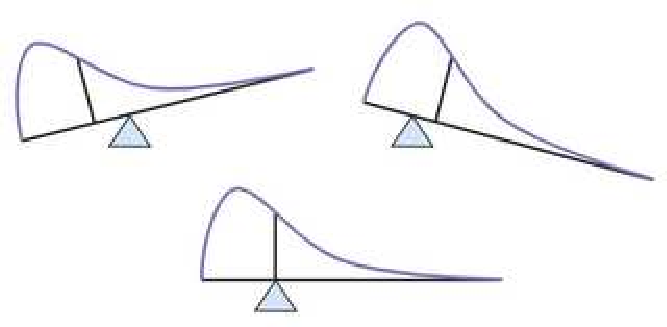
\includegraphics[width=.8\textwidth]{balance.pdf}
\end{center}
\end{frame}

\begin{frame}{Effects of Shifting, Reflection, and Scaling on the
Average}
\protect\hypertarget{effects-of-shifting-reflection-and-scaling-on-the-average}{}
Consider these four lists:

\begin{center}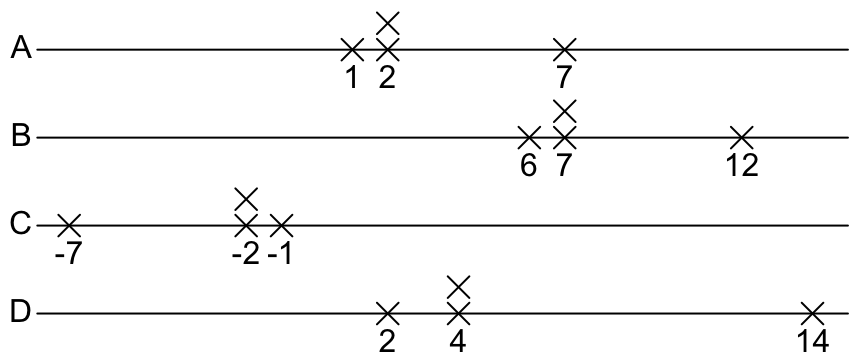
\includegraphics[width=0.75\linewidth]{ch04A_24spr_files/figure-beamer/torque5-1} \end{center}

\begin{enumerate}
\item
  How is list B related to list A? How is the average of list B related
  to the average of list A?\newline \smallskip
  \onslide<2->{\alert{The numbers shifted by 5, and so does their average.}}
\item
  Ditto, for C?\newline \smallskip
  \onslide<3->{\alert{The numbers changed sign, and so did their average.}}
\end{enumerate}
\end{frame}

\begin{frame}{}
\protect\hypertarget{section-1}{}
\begin{center}
\includegraphics[width=0.75\linewidth]{ch04A_24spr_files/figure-beamer/unnamed-chunk-5-1} \end{center}

\begin{enumerate}
\setcounter{enumi}{2}
\tightlist
\item
  Ditto, for D?\newline \smallskip
  \onslide<2->{\alert{The numbers doubled, and so did their average.}}
  \medskip
\end{enumerate}

\underline{General Rules}:

\begin{itemize}
\item
  If each element of a list is shifted by some constant, the average
  will be \textbf{shifted} by that constant.
\item
  If each element of a list is multiplied by some constant, the average
  will be \textbf{multiplied} by that constant.
\end{itemize}
\end{frame}

\begin{frame}{Another Measure of the Center: Median}
\protect\hypertarget{another-measure-of-the-center-median}{}
The \hl{median} of a numerical variable is a number such that half of
the observed value are smaller than it and half are larger than it.

\textbf{Ex 1}: Suppose a variable has 5 observed values: 4, 8, 3, 5, 12.

\begin{center}\small
\begin{tabular}{@{}rcccccc}
data   & $\to$ & 4 & 8 & 3 & 5 & 12\\[-2pt]
sorted & $\to$ & 3 & 4 & \only<1|handout:0>{5}\only<2->{\red{5}} & 8 & 12\\[-3pt]
       &       &   &   & \onslide<2->{\red{$\downarrow$}} &&\\[-3pt]
       &       &   &   \multicolumn{3}{c}{\onslide<2->{\red{Median}}}&

\end{tabular}
\end{center}

\textbf{Ex 2}: If the variable has one more observation: 4, 8, 3, 5, 12,
\red{100}.

\begin{center}\small
\begin{tabular}{@{}rccccccc}
data   & $\to$ & 4 & 8 & 3 & 5 & 12 & 100\\[-2pt]
sorted & $\to$ & 3 & 4 & \only<1-2|handout:0>{5}\only<3->{\red{5}} & \only<1-2|handout:0>{8}\only<3->{\red{8}} & 12 & 100\\
\end{tabular}
\end{center}

The median is thus \(\dfrac{5+8}{2}=6.5.\)
\end{frame}

\begin{frame}{Median is More Robust to Extreme Values Than Average}
\protect\hypertarget{median-is-more-robust-to-extreme-values-than-average}{}
\textbf{Example}. If the variable has a new 6th observation of value
100,

\begin{center}
4, 8, 3, 5, 12, \red{100}
\end{center}

The new average of the variable becomes \[
\frac{4+8+3+5+13+\red{$100$}}{6} = \frac{132}{6} = 22.
\]

\begin{center}
\begin{tabular}{l|cc}
Data & Mean & Median\\\hline
4, 8, 3, 5, 12      & 6.4 & 5\\\hline
4, 8, 3, 5, 12, 100 & 22  & 6.5
\end{tabular}
\end{center}

\textbf{The median is less affected by the extreme value (100) than the
average}. We say the median is more \red{robust} than the mean.
\end{frame}

\begin{frame}{Median and Average of a Histogram}
\protect\hypertarget{median-and-average-of-a-histogram}{}
The \textbf{median} divides the area of a histogram evenly.

\vspace{-6pt}

\begin{center}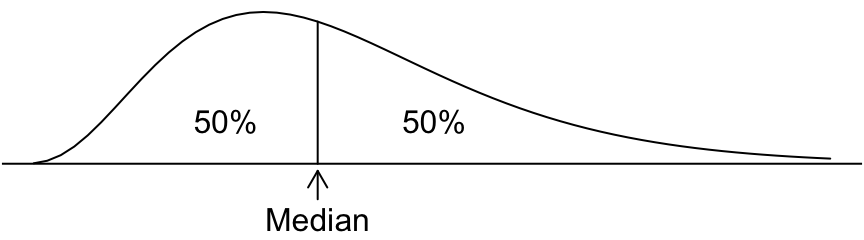
\includegraphics[width=0.75\linewidth]{ch04A_24spr_files/figure-beamer/median-1} \end{center}
\end{frame}

\begin{frame}{Average vs.~Median and Skewness}
\protect\hypertarget{average-vs.-median-and-skewness}{}
\begin{itemize}
\tightlist
\item
  In a symmetric distribution, Average \(\approx\) Median.

  \begin{itemize}
  \tightlist
  \item
    If exactly symmetric, then Average \(=\) Median.
  \end{itemize}
\item
  In a skewed distribution, the average is pulled toward the longer
  tail.
\end{itemize}

\begin{center}
\includegraphics[width=0.9\linewidth]{ch04A_24spr_files/figure-beamer/unnamed-chunk-6-1} \end{center}
\end{frame}

\begin{frame}{Measuring Spread: Standard Deviation (SD)}
\protect\hypertarget{measuring-spread-standard-deviation-sd}{}
Steps to compute the SD of the list 1,2, 2,7

\begin{enumerate}
\tightlist
\item
  Find the average of the list.
  \hid{2-}{$\displaystyle{\frac{1+2+2+7}{4}=3}$}
\item
  Find the deviations from average. \hid{3-}{$-2$, $-1$, $-1$, 4}
\item
  Square the deviations. \hid{4-}{$4$, $1$, $1$, 16}
\item
  Average the squared deviations. \onslide<5->{\alert{$\displaystyle
    \frac{4 + 1 + 1 + 16}{4} = \frac{22}{4}$}}
\item
  Take the square root.
  \onslide<6->{\alert{$$\text{SD} =\sqrt{22/4} \approx 2.3$$}}
\end{enumerate}

\begin{center}
\fboxrule=1pt
\fboxsep=10pt
\fbox{SD $=$
\begin{tabular}{c}
Root Mean Square (\textbf{RMS}) of the \\
deviations from the average of the list
\end{tabular}}
\end{center}
\end{frame}

\begin{frame}{Example}
\protect\hypertarget{example}{}
Each of the following lists has an average of 50. Which list has the
smallest SD? The largest?

\bigskip

A:
0,\hfill 20,\hfill 40,\qquad 50,\qquad 60,\hfill 80,\hfill,100\newline
\medskip B: 0,\hfill 48, 49, 50, 51, 52,\hfill,100\newline \medskip C:
0, 1, 2,\hfill 50,\hfill,98, 99,100\newline

What are the SDs?

\begin{center}
\begin{tabular}{l|ccc}
              & A & B & C  \\
              \hline
By eye        & \onslide<4->{\alert{middle}}   & \onslide<3->{\alert{smallest}}  & \onslide<2->{\alert{largest}}   \\
By calculator &\onslide<5->{\alert{32}} & \onslide<5->{\alert{27}} & \onslide<5->{\alert{45}}
\end{tabular}
\end{center}
\onslide<6->{\alert{List B shows that the SD pays considerable attention to large deviations.}}

\textbf{SD is very sensitive to extreme values.}
\end{frame}

\begin{frame}{Effects of Shifting, Reflection, and Scaling on the SD}
\protect\hypertarget{effects-of-shifting-reflection-and-scaling-on-the-sd}{}
Consider these four lists:

\begin{center}
\includegraphics[width=0.75\linewidth]{ch04A_24spr_files/figure-beamer/unnamed-chunk-7-1} \end{center}

\begin{enumerate}
\tightlist
\item
  How is the SD of list B related to that of list A?\newline
  \hid{2-}{The spread of a list is not affected by shifting. \centerline{SD of B $=$ SD of A}.}
\item
  Ditto, for C?\newline
  \hid{3-}{The spread of a list is not affected by reflection. $$\text{SD of C} = \text{SD of A}.$$}
\end{enumerate}
\end{frame}

\begin{frame}{}
\protect\hypertarget{section-2}{}
\begin{center}
\includegraphics[width=0.75\linewidth]{ch04A_24spr_files/figure-beamer/unnamed-chunk-8-1} \end{center}

\begin{enumerate}
\setcounter{enumi}{2}
\tightlist
\item
  Ditto, for D? \smallskip
  \onslide<2->{\alert{The spread doubled, and so did the SD.}}
\end{enumerate}

\underline{General Rule}:

\begin{itemize}
\item
  If each element of a list is shifted by some constant, the SD is
  \textbf{unchanged}.
\item
  If each element of a list is multiplied by some constant, the SD gets
  \textbf{multiplied} by the \textbf{absolute value} of that constant.
\end{itemize}
\end{frame}

\begin{frame}{Exercise}
\protect\hypertarget{exercise}{}
For list A, Average \(= 5\), SD \(=2.05\).\newline Please find the
averages and SDs for list B and list C respectively.

\vspace{-12pt}
\begin{center}\small
\tabcolsep=12pt
\renewcommand{\arraystretch}{1.1}
\begin{tabular}{@{}r|c|c|c}
\multicolumn{1}{@{}c}{} & \multicolumn{3}{c}{List}\\\cline{2-4}
 & A &  B &  C\\\hline
 & 4 & 24 & 40\\
 & 6 & 26 & 60\\
 & 8 & 28 & 80\\
 & 6 & 26 & 60\\
 & 5 & 25 & 50\\
 & 1 & 21 & 10\\
 & 7 & 27 & 70\\
 & 6 & 26 & 60\\
 & 5 & 25 & 50\\
 & 2 & 22 & 20\\\hline
Average & 5.00 & & \\\cline{2-4}
SD      & 2.05 & & \\\hline
\end{tabular}
\end{center}
\end{frame}

\begin{frame}{The 68\%- and 95\%-Rules}
\protect\hypertarget{the-68--and-95-rules}{}
Roughly 68\% (2 in 3) of the entries on a list are within 1 SD of the
average, the other 32\% are further away.

Roughly 95\% (19 in 20) of the entries on a list are within 2 SDs of the
average; the other 5\% are further away.

This is so for many lists, but not all.
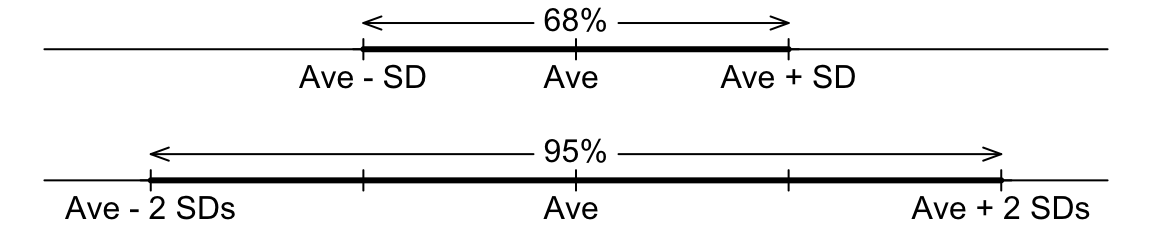
\includegraphics{ch04A_24spr_files/figure-beamer/rule6895-1.png}

\begin{itemize}
\tightlist
\item
  These rules work especially well for lists with \textbf{bell-shaped}
  histograms.
\item
  These rules work reasonably well for lists with unimodal, and not
  seriously skewed histograms.
\end{itemize}
\end{frame}

\begin{frame}{68\% Rule for the FEV Data}
\protect\hypertarget{rule-for-the-fev-data}{}
\vspace{-8pt}
\begin{center}\small
\tabcolsep=4pt
\begin{tabular}{lccrr}
                 &       &     &   & proportion within\\[-3pt]
Sex/Smoke        & Average  & SD & Count & \red{1 SD} from Ave\\\hline
Female Nonsmoker & 2.379 & 0.639 & 279 & $170/279 \approx 60.9\%$\\
Female Smoker    & 2.966 & 0.423 &  39 & $27/39 \approx 69.2\%$ \\
Male Nonsmoker   & 2.734 & 0.974 & 310 & $203/310 \approx 65.5\%$ \\
Male Smoker      & 3.743 & 0.889 &  26 & $17/26 \approx 65.4\%$ 
\end{tabular}
\end{center}

\vspace{-12pt}

\begin{center}
\includegraphics[width=0.85\linewidth]{ch04A_24spr_files/figure-beamer/unnamed-chunk-11-1} \end{center}
\end{frame}

\begin{frame}{95\% Rule for the FEV Data}
\protect\hypertarget{rule-for-the-fev-data-1}{}
\vspace{-8pt}
\begin{center}\small
\tabcolsep=4pt
\begin{tabular}{lccrr}
                 &       &     &   & proportion within\\[-3pt]
Sex/Smoke        & Average  & SD & Count & \red{2 SDs} from Ave\\\hline
Female Nonsmoker & 2.379 & 0.639 & 279 & $270/279 \approx 96.8\%$\\
Female Smoker    & 2.966 & 0.423 &  39 & $38/39 \approx 97.4\%$ \\
Male Nonsmoker   & 2.734 & 0.974 & 310 & $298/310 \approx 96.1\%$ \\
Male Smoker      & 3.743 & 0.889 &  26 & $24/26 \approx 92.3\%$ 
\end{tabular}
\end{center}

\vspace{-12pt}

\begin{center}
\includegraphics[width=0.85\linewidth]{ch04A_24spr_files/figure-beamer/unnamed-chunk-13-1} \end{center}
\end{frame}

\begin{frame}{Exercise}
\protect\hypertarget{exercise-1}{}
Is the SD of the histogram below closest to 5, 15, or 50?

\only<1| handout:0>{


\begin{center}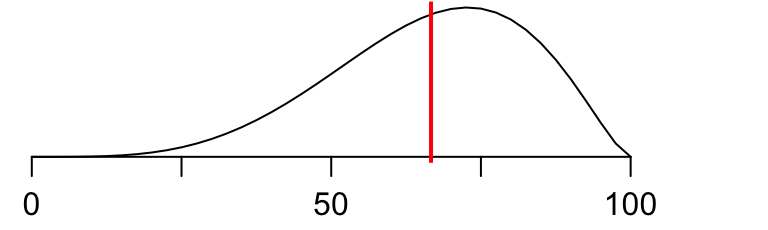
\includegraphics[width=0.8\linewidth]{ch04A_24spr_files/figure-beamer/S220RE0406A-1} \end{center}


}\only<2| handout:0>{


\begin{center}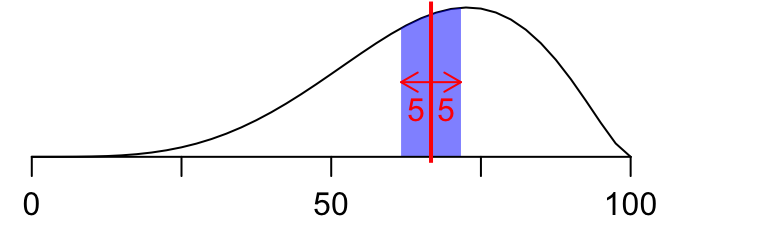
\includegraphics[width=0.8\linewidth]{ch04A_24spr_files/figure-beamer/S220RE0406A-2} \end{center}


}\only<3| handout:0>{


\begin{center}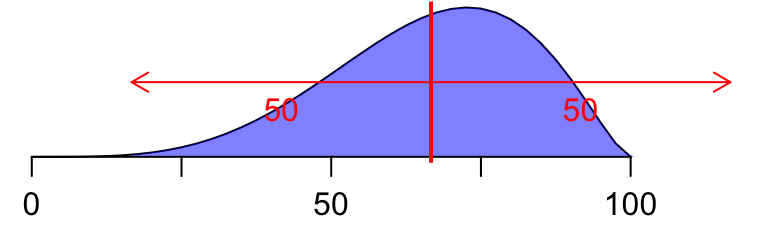
\includegraphics[width=0.8\linewidth]{ch04A_24spr_files/figure-beamer/S220RE0406A-3} \end{center}


}\only<4| handout:0>{


\begin{center}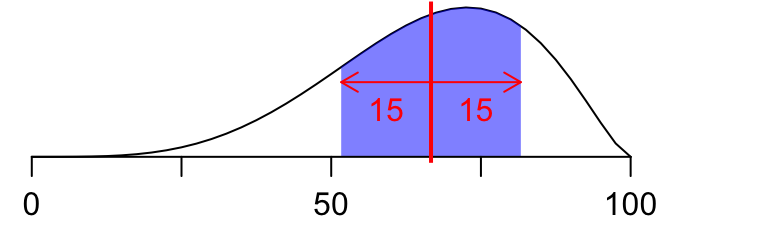
\includegraphics[width=0.8\linewidth]{ch04A_24spr_files/figure-beamer/S220RE0406A-4} \end{center}


}
\end{frame}

\begin{frame}{Exercise (68\%- and 95\%-Rules)}
\protect\hypertarget{exercise-68--and-95-rules}{}
Below are sketches of histograms for three lists. Match the sketch with
the description. Some descriptions will be left over. Give your
reasoning in each case.

\begin{center}
\begin{tabular}{clccl}
   (i) & ave $\approx$ 3.5, SD $\approx$ 1   &&   (iv) & ave $\approx$ 2.5, SD $\approx$ 1   \\
  (ii) & ave $\approx$ 3.5, SD $\approx$ 0.5 &&    (v) & ave $\approx$ 2.5, SD $\approx$ 0.5 \\
 (iii) & ave $\approx$ 3.5, SD $\approx$ 2   &&   (vi) & ave $\approx$ 4.5, SD $\approx$ 0.5
\end{tabular}
\end{center}

\begin{center}
\includegraphics[width=1\linewidth]{ch04A_24spr_files/figure-beamer/unnamed-chunk-14-1} \end{center}
\end{frame}

\begin{frame}{Mathematical Notation}
\protect\hypertarget{mathematical-notation}{}
\begin{itemize}
\item
  In mathematical notation, a generic list can represented as
  \[x_1,\, x_2,\, \ldots, x_n.\] Here \(x_1\) stands for the first
  element on the list, \(x_2\) for the second, \(\ldots\), and \(x_n\)
  for the last; \(n\) stands for the number of elements on the list.
\item
  The average of the generic list is \[
  \frac{\text{sum of the values}}{\text{how many there are}}
  = \frac{x_1  + x_2 + \cdots + x_n}{n}
  \] The average of \(x_1,x_2,\ldots,x_n\) is commonly denoted by
  \(\bar x\), read \red{$x$-bar}.
\end{itemize}
\end{frame}

\begin{frame}{Caution: Sample SD}
\protect\hypertarget{caution-sample-sd}{}
The SD of the generic list is the RMS deviation from average: \[
\text{SD} = \sqrt {\frac{ (x_1 - \bar x)^2 + (x_2 - \bar x)^2 +
\cdots + (x_n - \bar x)^2}{n}} 
\] Most calculators and statistical softwares compute the SD as the
slightly larger number
\[\text{sample SD} = \sqrt {\frac{ (x_1 - \bar x)^2 + (x_2 - \bar x)^2 +
\cdots + (x_n - \bar x)^2}{n-1}} \] called the \hl{sample SD}, commonly
denoted by \red{$s$}.\\
Thus \[\text{SD} = \sqrt{\frac{n-1}{n}} \, s =
\sqrt{\frac{\text{number of entries}- 1}
    {\text{number of entries}}}\, (\text{sample SD}).
\]
\end{frame}

\begin{frame}{Summary of Measures of Center \& Spread}
\protect\hypertarget{summary-of-measures-of-center-spread}{}
\begin{tabular}{@{}c|cccc}
       & Shifting & Scaling & Reflection & Sensitive \\[-2pt]
       & $x_i\rightarrow x_i+b$ & $x_i\rightarrow ax_i$ & $x_i\rightarrow -x_i$ & to extreme \\
       & for all $i$ & for all $i$ & for all $i$ & values?\\
\toprule
Average   & shifted by $b$ & Scaled by $a$ & change sign & Yes\\
$\bar{x}$ & $\bar{x}\rightarrow \bar{x}+b$ & $\bar{x}\rightarrow a\bar{x}$ &$\bar{x}\rightarrow -\bar{x}$ &\\
\midrule
Median & shifted by $b$ & Scaled by $a$ & change sign & No\\
\midrule
SD     & unchanged      & Scaled by $|a|$ & unchanged & Yes\\
       &                & SD $\rightarrow |a|\times\,$SD&&
\end{tabular}
\end{frame}

\end{document}
